% !TEX root = ../../commutative_algebra.tex

\newpage
\section{Hilbert's Nullstellensatz \& Krull's Intersection Theorem}

\subsection{Krull Dimension}

\begin{dfn}[Transcendence Degree]
Let $X$ be a topological space. A subset $Y \subseteq X$ is called irreducible if $Y$ is not a union of two proper closed subsets (note the difference between this and connected is these sets need not be disjoint). Otherwise, the subset is called reducible. The (combinatorial) dimension of $X$ is the sup of the longest chain of irreducible subsets. 
\end{dfn}

In particular, if $X$ is an affine algebraic variety then the subset $Y \subseteq X$ is irreducible. If not, it is a union of proper subvarieties. The dimension of $X$ is the sup of lengths of chains of irreducible subsets. 

\begin{ex}
Points are irreducible as $\dim(\{p\})=0$. In fact, $\dim(\{p_1,\cdots,p_n\})=0$.
\end{ex}

\begin{ex}
The set $Z(y-x^2)$ is ``clearly" irreducible in $\A_k^1$. We know $\dim Z(y-x^2) \geq 1$. The question is, is this dimension actually 1? The answer is yes - as one would expect - but we need more theory to prove it. This will follow from the next proposition as $k[x,y]/(y-x^2) \cong k[x]$, a domain.
\end{ex}

\begin{prop}
A variety $X \subseteq \A_k^n$ is irreducible if and only if $I(X)$ is prime. 
\end{prop}

\noindent Proof: Suppose that $X$ is irreducible and let $f,g \in k[x_1,\cdots,x_n]$ such that $f,g \in I(X)$. Let $Y_1=Z(I(X)+(f))$ and $Y_2=Z(I(X)+(g))$. We know that $Y_1,Y_2$ are subvarieties of $X$. We claim that $X=Y_1 \cup Y_2$. To prove $\subseteq$, let $p \in X$. Then we know that $(fg)(p)=0$ so that $f(p)=0$ and $g(p)=0$. So $p \in Y_1$ or $p \in Y_2$. We need also show that $Y_1,Y_2 \neq X$. As $X$ is an irreducible union of subvarieties, we know $X=Y_1$ or $X=Y_2$. If $X=Y_1$, then $f \in I(X)$ (as $X$ is among the zeros of $f$). Mutatis mutandis, if $X=Y_2$ then $g \in I(X)$. To prove $\supseteq$, assume that $X$ is reducible. We want to show that $I(X)$ is not prime so that we have proper subvarieties $Y_1,Y_2 \subsetneq X$ such that $X=Y_1 \cup Y_2$. Since $Y_1 \subsetneq X$, we have $I(X) \subseteq I(Y_i)$ for $i=1,2$. If $I(X)=I(Y_i)$, then $\ov{Y}_i=Z(I(Y_i))=Z(I(X))=\ov{X}$ and $Y_i,X$ are closed so that this gives equality. Then $I(X) \subsetneq I(Y_i)$ for $i=1,2$. Take $f_i \in I(Y_i) \setminus I(X)$. Then $f_1f_2 \in I(Y_1)I(Y_2) \subseteq I(Y_1) \cap I(Y_2)=I(Y_1 \cup Y_2)=I(X)$ so that $I(X)$ is not prime. \qed \\

\begin{dfn}[Krull Dimension]
The Krull dimension of a commutative unital ring $R$ is
\[
\dim R=\sup\{n\;|\; \text{ there is a chain of prime ideals of } R, \; p_0 \subsetneq p_1\subsetneq \cdots \subsetneq p_n\}
\]
\end{dfn}

\begin{cor}
$\dim X=\dim k[x]$ for a variety $X \subseteq \A_k^n$.
\end{cor}

\noindent Proof: $Y \subseteq X$ is an irreducible subvariety if and only if $I(Y) \supseteq I(X)$ is a prime ideal. \qed \\

\begin{dfn}[Height]
The height of a prime ideal $p \in \spec R$ is
\[
\htt p \defeq \sup \{n\;|\; \text{there is a chain of prime ideals in }R, \; p_0 \subsetneq p_1 \subsetneq \cdots \subsetneq p_n=p\}
\]
\end{dfn}

We know that $\spec(R_p)=\{q \in \spec R\;|\; q \subseteq p\}$. That is, $\spec(R_p)=\{q \in \spec R\;|\; q \cap (R/p) = \emptyset\}$. This is the same as $\htt p=\dim R_p$. We know also that $\spec(R/p)=\{q \in \spec R\;|\; q \supseteq p\}$. So $\htt p+\dim R/p \geq \dim R$. Notice the sum on the left is the sup of the lengths of chains containing $p$. Strict inequality can occur if in the inclusion diagram looks like the following:

\begin{figure}[H]
   \centering
   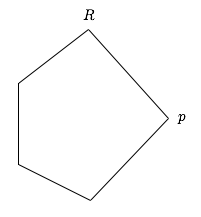
\includegraphics[width=1.5in]{diag.png} 
\end{figure}

Then notice we have $\htt p=1$, $\dim R/p=1$ but $\dim R=3$. 

\begin{dfn}[Catenary]
We say that $R$ is catenary if all saturated chains of primes between any two primes have the same length. Recall a saturated chain is one which cannot be refined. 
\end{dfn}

\begin{thmm}[Ratliff]
If $R$ is catenary then $\htt p+\dim R/p=\dim R$ for all primes $p \in \spec R$. Furthermore, any affine algebraic variety over a field is catenary. 
\end{thmm}

\noindent Proof: If $(f)$ is nonzero prime, then $(0) \subseteq (f)$ is a chain of length 1 so $\dim R \geq 1$. To show that $\dim R \leq 1$, we need to show that if $(f) \leq (g)$ for nonzero primes then we have equality, so we cannot extend the chain. Since $(f) \subseteq (g)$, then $f=rg$ for some $r$ so that $rg \in (f)$. As $(f)$ is prime, $r \in (f)$ or $g \in (f)$. We show that $r \notin (f)$: if $r=sf$, then $f=rg=sfg$ so that $(1-sg)f=0$. But then $f=0$, a contradiction. So $1-sg=0$ so that $1=sg$, showing that $(g)$ is not prime. \qed \\

Note that the converse is false as $\dim \Z[\sqrt{-5}]=1$ but this is not a UFD so that it is trivially not a PID. 

The first example of a non-catenary ring is due to Nagata in the 1950s and is not trivial. One should note that height was once called codimension and is still sometimes referred to as this - most notably in algebraic geometry. 

\begin{ex} To see some examples of this theorem:
\begin{enumerate}[(i)]
\item We have $\spec \Z=\{(0)\} \cup \{(p)\}_{p \text{ prime}}$. Each ideal $(p)$, where $p$ is prime, contains $(0)=\{0\}$ and no such ideal contains the other so that $\dim \Z=1$.

\item Generally, if $R$ is a PID that is not a field, then $\dim R=1$. 

\item If $k$ is a field then $\dim k=0$ (as it has a ``tiny" $\spec$). More generally, any artinian ring is 0-dimensional. 
\end{enumerate}
\end{ex}

Recall the following important result:

\begin{thmm}[Hopkins-Levitski Theorem]
Any artinian ring $R$ is noetherian. 
\end{thmm}

\begin{rem} There are a few important notes on the Hopkins-Levitski Theorem: 
\begin{enumerate}[(i)]
\item The converse of the Hopkins-Levitski Theorem: take $\Z$ or $k[x]$.
\item The Hopkins-Levitski Theorem is false for modules.
\item The proof of the Hopkins-Levitski Theorem shows more: if $R$ is an artinian ring:
\begin{itemize}
\item as a $R$-module, $R$ has finite length
\item $R$ has finitely many maximal ideals $\fm_1,\fm_2,\cdots,\fm_n$ and $J\defeq \cap \text{ max ideals}=\fm_1\cdots\fm_n$, where the last equality holds by the Chinese Remainder Theorem (if they are comaximal, this is obvious as they are maximal), and $J$ is nilpotent with $J=\nil R$. 
\end{itemize}
\end{enumerate}
\end{rem}

\begin{prop}
Let $R$ be a commutative noetherian ring, then $R$ is artinian if and only if $\dim R=0$.
\end{prop}

\noindent Proof: Assume that $R$ is artinian. By the Hopkins-Levinsky Theorem, $J$ is the jacobson radical of $R$. We know that $R$ has finitely many maximal ideals and $J$ is nilpotent. Then $J^s=0$ for some $s \geq 0$. Then we have $J^s \subseteq p$ for all $p \in \spec R$. This says that $J \subseteq p$. But we know that $J=\fm_1\cdots \fm_n$ so that $\fm_i \subseteq p$ for some $i$. Then $\spec R=\{\fm_1,\cdots,\fm_n\}$. In particular, there are no containments. 

If $\dim R=0$, then every prime ideal ideal is both maximal and minimal in $\spec R$. So every $p \in \spec R$ is a minimal prime of $(0)$. As $R$ is noetherian, the set $\spec R$ is finite. Suppose $\spec R=\{\fm_1,\cdots,\fm_n\}$. Then using Krull's Theorem, $\nil R=\cap_{p \in \spec R} p=\cap_{i=1}^n \fm_i=J$. In particular, we have $J=\fm_1\cdots\fm_n$ (by the Chinese Remainder Theorem). We have composition series for $R$
\[
R \supset \fm_1 \supset \fm_1 \fm_2 \supset \cdots J \supset J\fm_1 \supset J\fm_1\fm_2 \supset \cdots \supset J^2 \supset \cdots \supset J^s=0
\]
so that $R$ has finite length so that $R$ is artinian. \qed \\

\begin{ex}
$\dim(k[x_1,\cdots,x_n])=\dim \A_k^n=n$. To see that $\dim \geq n$, look at the inclusion $(0) \subsetneq (x_0) \subsetneq (x_0,x_1) \subsetneq \cdots \subsetneq (x_0,\cdots,x_n)$. To prove the other inequality, we need more theory.
\end{ex}

\begin{dfn}[Transcendence Basis]
Let $L/K$ be a field extension. A transcendence basis for an extension $L/K$ is a subset $B \subseteq L$ such that 
\begin{enumerate}[(i)]
\item $B$ is algebraically independent over $K$; that is, there does not exist a polynomial $f \in k[x_1,\cdots,x_n]$ such that $f(b_1,\cdots,b_n)=0$ for some $b_i \in B$. 
\item If $L$ is algebraic over $K(B)$.
\end{enumerate}
The cardinality of the basis $B$ is the transcendence degree of $L/K$, denoted $\tdeg(L/K)$ or $\tdeg_k(L)$.
\end{dfn}

One should show that this is uniquely defined - which it is - but we shall take this on faith. Observe that $\tdeg_k(L)$ is the cardinality of a maximal algebraic independent set.

\begin{ex}
Let $x_1,\cdots,x_n$ be indeterminant over $k$. We have $\tdeg_k k(x_1,\cdots,x_n)=n$. Then $k(x_1,\cdots,x_n)$ is purely transcendental over $k$, i.e. $L=K(B)$.
\end{ex}

\begin{ex}
If $L/K$ is an algebraic extension, then $\tdeg_k L=0$. 
\end{ex}

\begin{ex}
Let $S=k[x,y,z]$ and $f=xy-z^2 \in S$. One can show that $f$ is irreducible. Since $f$ is a UFD, we know that $f$ irreducible implies that $f$ is prime. So $R=k[x,y,z]/(f)$ is an integral domain. Set $L=Q(R)$. We claim that $\tdeg L/K=2$. Note that $Z(f) \subseteq \A_k^3$, the surface of a cone. To show this, we have $L=k(\ov{x},\ov{y},\ov{z})$ but not algebraically independent as $\ov{z}^2-\ov{x} \ov{y}=0$ in $L$. We shall show that $\{\ov{x},\ov{y}\}$ is a transcendence basis. Observe $L$ is algebraic over $k(\ov{x},\ov{y})$ since $\ov{z}$ is a root of $t^2-\ov{x}\ov{y}$. Then we have a $p(r,s) \in k(r,s)$ such that $p(\ov{x},\ov{y})=0$. But then $p(\ov{x},\ov{y})=\ov{p(x,y)}$. This means that $p(x,y)$ is a multiple of $(xy-z^2)$ in $k(x,y,z)$. But arguing by polynomial degree of $p(x,y)$ in $z$ that this is false so that $p(x,y)=0$.
\end{ex}

\begin{lem}[Lemma A]
Let $L/K$ be an algebraic field extension and $\alpha_1,\cdots,\alpha_n \in L$. Define $\phi: k[x_1,\cdots,x_n] \to L$ via $\phi(x_i)=\alpha_i$. Then $\ker \phi$ is a maximal ideal can be generated by $n$ polynomials $f_1(x_1),f_2(x_1,x_2),\cdots,f_n(x_1,\cdots,x_n)$ with each $f_i$ monic in $x_i$. 
\end{lem}

\noindent Proof: We know that $\im \phi$, $k[\alpha_1,\cdots,\alpha_n]$, is $k(\alpha_1,\cdots,\alpha_n)$ since each $\alpha_i$ is algebraic over $k$. This is a field so $k[x_1,\cdots,x_n]/\ker \phi \cong \im \phi$ so that $\ker \phi$ is a maximal ideal. We now construct the $f_i$'s inductively. 

Let $f_1(x_1)$ be the minimal polynomial of $\alpha_1$ over $k$. Then $k[\alpha_1] \cong k[x]/f_1(x)$, which is a field. This is isomorphic to $k(\alpha_1)$. Now $g_2(x) \in k(\alpha_1)[x]$ be the minimal polynomial for $\alpha_2$ over $k(\alpha_1)$. Since $k(\alpha_1)=k[\alpha_1]$, the coefficients of $g_2$ are polynomials in $\alpha_1$. So there is a $f_2(x_1,x_2) \in k[x_1,x_2]$ so that $k(\alpha_1,\alpha_2)=k(\alpha_1)[x_2]/f_2(\alpha_1,\alpha_2)$. We want to show that this is isomorphic to $k[x_1,\cdots,x_n]/(f_1,\cdots,f_n)$. Suppose that $p(x) \in \ker \phi$, i.e. $p(x_1,\cdots,x_n) \in k[x_1,\cdots,x_n]$ and $p(\alpha_1,\cdots,\alpha_n)=0$. 

We know that $f_n(\alpha_1,\cdots,\alpha_{n-1},x_n)$ be the minimal polynomial of $\alpha_n$ over a field $k(\alpha_1,\cdots,\alpha_{n-1})$. So $p$ is a multiple of $f_n$, i.e. $p(\alpha_1,\cdots,\alpha_{n-1},x) \in (f_n(\alpha_1,\cdots,\alpha_{n-1},x_n))$ as a polynomial in one variable $x_n$ over the field $k(\alpha_1,\cdots,\alpha_{n-1})$. Use the division algorithm for a polynomial in one variable in $k[x_1,\cdots,x_{n-1}]$ to write $p(x_1,\cdots,x_n)=q_nf_n+r_n$. Plugging in $x_i=\alpha_i$ for $i=1,2,\cdots,n-1$. We know that as $p(\alpha_1,\cdots,\alpha_{n-1},x) \in (f_n(\alpha_1,\cdots,\alpha_{n-1},x_n))$, we have $r_n=0$. But then $r_n(\alpha_1,\cdots,\alpha_{n-1},x_n)=0$. Then $r_n(\alpha_1,\cdots,\alpha_{n-2},x_{n-1},x_n) \in (f_{n-1}(x_1,\cdots,x_{n-1}))$ sine $k(\alpha_1,\cdots,\alpha_{n-1}) \cong k(\alpha_1,\cdots,\alpha_{n-2})[x_{n-1}]/(f_{n-1}(\alpha_1,\cdots,\alpha_{n-2},x_{n-1}))$. 

We repeat the argument, $r_n=q_{n-1}f_{n-1}+r_{n-1}$ as polynomials in $x_{n-1}$ over $k[x_1,\cdots,x_{n-2}]$ and plug in $\alpha_1,\cdots,\alpha_{n-2}$, et cetera. We get $p=q_nf_n+r_n,r_n=q_{n-1}f_{n-1}+r_{n-1},\cdots$. After $n$ steps, we have $p=\sum_{i=1}^n q_i+f_i+r_1(x_1,\cdots,x_n)$. So $r_1=0$ os that $p \in (f_1,\cdots,f_n)$. [Note that each step, $r_j(x_1,\cdots,x_n) \in (f_{j-1}(x_1,\cdots,x_{j-1}))$ after plugging in $\alpha_1,\cdots,\alpha_{j-2}$ so we write $r_j=q_{j-1}f_{j-1}+r_{j-1}$. So when $j=2$, we have $r_2 \in (f_1(x_1))$ and after plugging in 0 $\alpha$'s, we have $r_2=q_1f_1$.] \qed \\

\begin{lem}[Lemma B]
Let $k$ be a field and $R$ be a finitely generated $k$-algebra which is a domain. If $\tdeg_k Q(R)>0$ then $R$ is not a field. Therefore, if $R$ is a field then $\tdeg_k Q(R)=0$. 
\end{lem}

\noindent Proof: Let $\alpha_1,\cdots,\alpha_n \in R$ be elements which generate $R$ as an algebra over $k$. So we have $R=k[\alpha_1,\cdots,\alpha_n]$ and $Q(R)=k(\alpha_1,\cdots,\alpha_n)$. The set $\{\alpha_1,\cdots,\alpha_n\}$ contains a transcendence basis, say $\{\alpha_1,\cdots,\alpha_r\}$. Then $\{\alpha_{r+1},\cdots,\alpha_n\}$ are algebraic over the field $k[\alpha_1,\cdots,\alpha_r]=K$. By Lemma A, we can write $Q(R)=K[\alpha_{r+1},\cdots,x_n]/(f_{r+1}(x_{r+1}),\cdots,f_{n-r}(x_{r+1},\cdots,x_n))$. Set $d_i=\deg_{x_i} f_i$ for $i=r+1,\cdots,n$. Then $[k(\alpha_{r+1},\cdots,\alpha_{i+1}): k(\alpha_{r+1},\cdots,\alpha_i)]=d_i$. Now $K=k(\alpha_1,\cdots,\alpha_r)=Q(k[\alpha_1,\cdots,\alpha_r])$. So $k=k[\alpha_1,\cdots,\alpha_r]$ since they are transcendental. Coefficients in $K$ of the $f_i$'s have denominators in $k[\alpha_1,\cdots,\alpha_r]$. We get $g \in k[\alpha_1,\cdots,\alpha_r]$ so that $gf_i \in k[\alpha_1,\cdots,\alpha_r][x_{r+1},\cdots,x_n]$. Set $B=k[\alpha_1,\cdots,\alpha_r,1/g]$. 

We claim that $R[1/g]=B[\alpha_{r+1},\cdots,\alpha_r]$ is a finitely generated free $B$-module. We want to show that if $r>0$ then $R$ is not a field. If $R$ were a field then $g \in R$ so that $1/g \in R$ so that $R[1/g]=R$ is a finitely generated free $B$-module. But then $B$ cannot have any proper nonzero ideals. If it had one, $I \subseteq B$ is a proper nonzero ideal, then $IR=R$ as $R$ is a field so that $R/IR=0$. But by the above claim, $R/IR=B^n/IB^n \cong (B/I)^n \neq 0$ as $I$ is proper. Then $B$ is a field. Now $B$ contains a polynomial ring $k[\alpha_1,\cdots,\alpha_r]$ in $r$ variables so that it contains infinitely many irreducibles not dividing $g$. If $h$ is one of those then $1/h \notin k[\alpha_1,\cdots,\alpha_r,1/g]=B$ so that $B$ cannot be a field. If $r \geq 1$, then $B$ cannot be a field so that $R$ cannot be a field. 

It only remains to verify the claim. We show that $\{\alpha_{r+1}^{e_{r+1}},\alpha_{r+2}^{e_{r+2}},\cdots,\alpha_n^{e_n}\;|\; 0 \leq e_i<d_i\}$ is a basis for $R[1/g]$ over $R$. Every element of $R[1/g]$ is a basis of the form $p(\alpha_{r+1},\cdots,\alpha_n)$ for some $p(x_{r+1},\cdots,x_n) \in B[x_{r+1},\cdots,x_n] \subseteq k[x_{r+1},\cdots,x_n]$. If $\deg P$ in $x_i>d_i$, we can use the division algorithm (since $f_i$ is monic in $x_i$) to replace $p$ by something else equivalent of smaller degree equivalent module the $f$'s of smaller degree. Then this set spans $R[1/g]$. The basis is linearly independent over $k(\alpha_1,\cdots,\alpha_r)$, by more elementary field theory, hence over $R$ (by passing to the quotient field). \qed \\

\begin{thmm}
Let $R$ be a finitely generated algebraic extension over a field $k$ and assume $R$ is a domain. Then $\dim R=\tdeg_k Q(R)$.
\end{thmm}

\noindent Proof: Let $L=Q(R)$ and $r=\tdeg_k L$. Write $R=k[x_1,\cdots,x_n]/p$ for some $p \in \spec R$. First, we show that $r \geq \dim R$. It suffices to show $p \subsetneq q$ and $\tdeg_k Q(k[x_1,\cdots,x_n]/p) > \tdeg Q(k[x_1,\cdots,x_n]/q)$. We have a surjective map $k[x_1,\cdots,x_n]/p \to k[x_1,\cdots,x_n]/q$. So any transcendence basis for the left serves as a transcendence basis for the right as a generator up to an algebraic extension. Assume that equality holds. Write $k[x_1,\cdots,x_n]/p =k(\alpha_1,\cdots,\alpha_n)$. We have $k[x_1,\cdots,x_n]/q=k[\beta_1,\cdots,\beta_n]$. Assume that both fields have transcendence degree $r$ over $k$ and reorder the $\beta$'s such that the first $r$ of them form a transcendence basis. 

Then $\alpha_1,\cdots,\alpha_r$ are also a transcendence basis as any polynomial vanishing on $\alpha_1,\cdots,\alpha_r$ would vanish on the $\beta$'s. Set $W=k[x_1,\cdots,x_r] \setminus \{0\}$. We claim $p \cap W=q \cap Q=\emptyset$. If something is in the left side, we can plug in the $\alpha$'s to obtain that is 0. We get something similar on the right side by plugging in the $\beta$'s. So both $p,q$ survive in $k[x_1,\cdots,x_n]_W=k(x_1,\cdots,x_r)[x_{r+1},\cdots,x_n]$. But now 
\[
k[x_1,\cdots,x_n]_W/pk[x_1,\cdots,x_n]_W=(k[x_1,\cdots,x_n]/p)_W=k[\alpha_1,\cdots,\alpha_n]_W=k(\alpha_1,\cdots,\alpha_r)[\alpha_{r+1},\cdots,\alpha_n]
\]
But this is a field as $\alpha_{r+1},\cdots,\alpha_n$ are algebraic over $k(\alpha_1,\cdots,\alpha_r)$. So $p$ must be maximal in $k[x_1,\cdots,x_n]_W$, a contradiction. Then $p \subsetneq q$ and $q \cap W =\emptyset$ so that $r \geq \dim R$. 

We show $r \leq \dim R$ by induction on $r$. If $r=0$, then $R$ is a field by Lemma B or $r=0$ and $\dim R \geq 0$. If $r>0$, write $R=k[\alpha_1,\cdots,\alpha_n]$ with at least $\alpha_i$ transcendental over $k$. Set $W=k[x_1]\setminus \{0\}$. Write $R=k[x_1,\cdots,x_n]/p$. We know $W \cap p=\emptyset$ and $k[x_1,\cdots,x_n]_W=k(x_1)[x_2,\cdots,x_n]$ so 
\[
R_W=k[x_1,\cdots,x_n]_W/pk[x_1,\cdots,x_n]_W \cong k(\alpha_1)[\alpha_2,\cdots,\alpha_n] 
\]
has transcendental degree over $k(\alpha_1)$ one less, namely $r-1$. Then via induction we obtain $\dim(k[x_1,\cdots,x_n]_W/pk[x_1,\cdots,x_n]_W) \geq r-1$. Then we get a chain of primes in $k[x_1,\cdots,x_n]_W$ starting with $q_0 \defeq pk[x_1,\cdots,x_n]_W$, i.e. $q_1 \subsetneq \cdots \subsetneq q_{r-1}$. We look at their preimages in $k[x_1,\cdots,x_n]$
\[
p=p_0 \subsetneq p_1 \subsetneq \cdots \subsetneq p_{r-1}
\]
with $W \cap p_i = \emptyset$. In particular, $x_1 \notin p_i$ for all $i$. So the image of $x_1$ in $k[x_1,\cdots,x_n]/p_{r-1}$ which maps $\alpha_1$ in $R$ is transcendental. Then by Lemma B, $k[x_1,\cdots,x_n]/p_{r-1}$ is not a field. So $p_{r-1}$ is not maximal so we can extend the chain of primes $\{p_i\}_{i=1}^{r-1}$ by at least 1 more step. \qed \\

\begin{thmm}
Let $\fm$ be a maximal ideal of $k[x_1,\cdots,x_n]$ and $K=k[x_1,\cdots,x_n]/\fm$ be the residue field. Then $K$ is algebraic over $k$. Furthermore, by Lemma A, we can write $\fm=(f_1,\cdots,f_n)$ for polynomials $f_1,\cdots,f_n$. In particular, if $k$ algebraically closed then $\fm=(x_1-a_1,\cdots,x_n-a_n)$ for some point $(a_1,\cdots,a_n) \in \A_k^n$. 
\end{thmm}

\noindent Proof: Let $\alpha_1,\cdots,\alpha_n$ be the images of $x_1,\cdots,x_n$ in $k$. Then $K=k[\alpha_1,\cdots,\alpha_n]$ is a field. By Lemma B, $\tdeg_k B=0$, i.e. $K/k$ is algebraic. For the last assertion, suppose that $k=\ov{k}$. Then $k$ has no algebraic extension so $\ov{K}=K$. Then for all $i$, there is $a_i \in k$ such that $x_i \equiv a_i \mod \fm$. So $(x_1-a_1,\cdots,x_n-a_n) \subseteq \fm$, this is a maximal ideal as $k[x_1,\cdots,x_n]/(x_1-a_1,\cdots,x_n-a_n)$ (killing by this ideal, we have $k(a_1,\cdots,a_n)=k$) so that $\fm=(x_1-a_1,\cdots,x_n-a_n)$ by maximality. \qed \\

\subsection{Nullstellensatz}

\begin{thmm}[Hilbert's Nullstellensatz]
Let $k$ be an algebraically closed field. Then
\begin{enumerate}[(i)]
\item If $Z(I)=\emptyset$ for some $I \subseteq k[x_1,\cdots,x_n]$, then $1 \in I$.
\item $I(Z(I))=\sqrt{I}$
\end{enumerate}
\end{thmm}

\noindent Proof: 
\begin{enumerate}[(i)]
\item Suppose $1 \notin I$, i.e. $I \neq R$. Then $I$ is contained in some maximal ideal, $\fm$, i.e. $I \subset \fm$. By the preceding theorem, we know that $\fm=(x_1-a_1,\cdots,x_n-a_n)$. Then every polynomial in $I$ vanishes at the point $(a_1,\cdots,a_n)$ so that $Z(I) \neq \emptyset$. 

\item We know that $I \subseteq I(Z(I))$ and that $I(Z(I))$ is a radical ideal. So $\sqrt{I} \subseteq I(Z(I))$. We need only show the other containment. Let $f \in I(Z(I)) \subseteq k[x_1,\cdots,x_n]$. Consider the ideal $J=I+(1-yf) \in k[x_1,\cdots,x_n,Y]$ (this is called ``the trick of Ralomowitch"). If $p=(a_1,\cdots,a_n,b) \in \A_k^{n+1}$ is $Z(J)$ (notice this means that the points of $Z(J)$ never vanish on $I$ by the construction of $J$), then $(a_1,\cdots,a_n) \in Z(I)$. This shows $f(a_1,\cdots,a_n) \in Z(I)$. Then $(1-yf)(p)=1$, a contradiction to the fact that $p \in Z(J)$.

But then $J$ must be the whole ring, i.e. $J=k[x_1,\cdots,x_n]$. Then $1 \in J$ so we can write $1=\sum p_i(x_1,\cdots,x_n,Y)g_i(x_1,\cdots,x_n)+h(x_1,\cdots,x_n,y)(1-yf(x_1,\cdots,x_n))$. Putting in any number from $\A_k^n$ we always obtain a degree 0 piece (the 1 on the left side). Choosing additionally $y=1/f(x_1,\cdots,x_n)$ then $1=\sum p_i(x_1,\cdots,x_n,1/f(x))g_i(x_1,\cdots,x_n)$. Clearing denominators with a sufficiently large power of $f$, say $N$, we have $f^N=\sum p_i(x_1,\cdots,x_n)g_i(x_1,\cdots,x_n) \in I$.

\end{enumerate}
\qed \\

Now that we have shown the Nullstellensatz, we head towards our next long term goal: to prove the Krull Intersection Theorem (1930s). 

\subsection{Krull's Principle Ideal Theorem}

\begin{lem}[Krull's Principle Ideal Theorem, Base Case]
If $R$ is a noetherian ring and $x \in R$. Let $p$ be a minimal prime of $(x)$, i.e. $(x) \subseteq p$ and there is not $q$ with $(x) \subseteq p \subseteq p$. Then $\htt p \leq 1$. 
\end{lem}

\noindent Proof: Notice if $x$ is a unit, then $(x)=R$ and there are no such $p$'s. We can let $p$ be a minimal prime of $(x)$ (as $x$ is not a unit). If $p$ contains no primes, we are done. Assume $p \supsetneq q$. We want to show that $q$ has height 0, i.e. contains no other primes. Equivalently, show $\dim R_q=0$ (because the height is the same as the dimension of the localization). So we look at the reduction. In $R_p$, we still have $(x)R_p \subseteq pR_p$ and $qR_p \subset pR_p$. If we can show $qR_p$ has height 0, then $\htt q=0$. 

In other words, we may assume that $R$ is a local ring with unique maximal ideal $p$ (that is, localize and replace $R$ by $R_p$). Then in $R/(x)$ (this is the new $R$ - $R_p$), $p$ (the image of $p$) is maximal but also minimal over $(x)$. So there are no primes between $p$ and $x$. So $p$ is minimal in $R/(x)$. In particular, $\dim R/(x)=0$. Then $R/(x)$ is artinian. Recall the symbolic powers of $q$: $q^{(n)}\defeq q^nR_q \cap R$. Now $p$ is minimal over $(x)$ and $q \subset p$. In particular, $x \notin q$. Look at $q^{(n)}+(x)$. We then have $p \supset q^{(n)}+(x) \supset (x)$ and $p \supset q$. We know that $q^{(n+1)} \subseteq q^{(n)}$. So $q^{(n+1)}+(x) \subseteq q^{(n)}+(x)$. Since $R/(x)$ is artinian, this gives a descending chain of ideals which then must stabilize, say at $N$. 

Then $q^{(N+1)}+(x)=q^{(N)}+(x)$ for some $N$. So for every $f \in q^{(n)}$, there exists $g \in q^{(n+1)}$ and $a \in R$ such that $f=g+ax$. But then $ax=f-g \in q^{(N)}$. But $q^{(N)}$ is a primary ideal. So $a \in q^{(N)}$ or $x \in \sqrt{q^{(N)}}=q$ (that is, $x^N \in q^{(N)}$). But $x \in q$ yields a contradiction so that $a \in q^{(N)}$. So in fact, $q^{(N)} \subseteq q^{(N+1)}+q^{(N)}x$. In the ring $R/q^{(N+1)}$, this says $\ov{q^{(N)}} \subseteq \ov{q^{(N)}x}$. This is a problem as Nakayama's Lemma states that this only occurs if $\ov{q^{(N)}}=0$, i.e. $q^{(N)}=q^{(N+1)}$. Then $q^NR_q=q^{N+1}R_q$ so that by Nakayama's Lemma, $q^NR_q=0$. Then as this is a maximal ideal of $R_q$ and is nilpotent, $\dim R_q=0$, as desired. \qed \\

\begin{ex}
Let $R=k[x,y]/(x^2,xy,y^2)$. Then $\spec R=\{(x,y)\}$. In particular, $(x,y)$ is a maximal ideal but also minimal (over any element chosen) and has height 0.
\end{ex}

We now show the most general version of Krulls Principle Ideal Theorem. 

\begin{thmm}
Let $R$ be noetherian and $x_1,\cdots,x_n \in R$. Let $p$ be the minimal prime of $x_1,\cdots,x_n$. Then $\htt p \leq n$. 
\end{thmm}

\noindent Proof: We use the same reduction as before - localize at $p$ to assume that $R$ is local with maximal ideal $p$. Now as before $R/(x_1,\cdots,x_n)$ has only one prime ideal, so it is artinian. In particular, some power of $p$ (as the powers of $p$ form a descending sequence) is contained in $(x_1,\cdots,x_n)$ (as this sequence descends to 0 in $R/(x_1,\cdots,x_n)$). Let $q \subset p$. We have to show that $\htt q \leq n-1$. We shall show this via induction. We need to show that $q$ is minimal over some $(n-1)$-generated ideal: $(y_1,\cdots,y_{n-1})$. We may assume there are no primes between $p$ and $q$. 

As before, since $p$ is minimal over $(x_1,\cdots,x_n)$ and in fact one we have $x_i \notin q$ for some $i$. Renumber so that this $x_i$ is $x_n$. Then we look at $q+(x_n) \subset p$. We claim this is minimal over $p$. If $q+(x_n) \subset p' \subset p$, then $p'$ is between $q$ and $p$ so that $p'$ is minimal over $q+(x_n)$. But then in $R/q+(x_n)$, $\ov{p}$ is nilpotent. This forces $\ov{(x_1,\cdots,x_n)}$ to be nilpotent. So for $i=1,2,\cdots,n-1$, $x_i^t=y_i+a_ix^n$ and $a_i \in R$ and $y_i \in q$. Take $t$ sufficiently large show that all the $y$'s have this property. It remains to show that $q$ is minimal over $(y_1,\cdots,y_n)$. 

Observe that $y_i \in q$. Some power of $p$ is contained in $(x_1,\cdots,x_n)$ and some power of $(x_1,\cdots,x_n)$ is in $(y_1,\cdots,y_{n-1},y_n,x_n)$. Passing to $R/(y_1,\cdots,y_n)$, $\ov{p}$ is nilpotent. In $R/(y_1,\cdots,y_{n-1})$, $\ov{p}$ is minimal over $(x_n)$. By Krull's Theorem, this implies that $\ov{p}$ has height at most 1 in $R/(y_1,\cdots,y_n)$. But $\ov{q}$ is strictly contained in $\ov{p}$ so that $\htt \ov{q}=0$ in $R/(y_1,\cdots,y_{n-1})$. Hence, $q$ is maximal over $(y_1,\cdots,y_{n-1})$ in $R$. \qed \\

\begin{cor}
$\dim k[x_1,\cdots,x_n]=n$
\end{cor}

\noindent Proof: First, note that $\dim(k[x_1,\cdots,x_n]) \leq n$ as $\dim(k[x_1,\cdots,x_n])=\dim \A_k^n=n$. To see that $\dim \geq n$, look at the inclusion $(0) \subsetneq (x_0) \subsetneq (x_0,x_1) \subsetneq \cdots \subsetneq (x_0,\cdots,x_n)$. Lemma A implies that any maximal ideal of $k[x_1,\cdots,x_n]$ can be generated by polynomials $f_1,\cdots,f_n$ so any maximal ideal of $k[x_1,\cdots,x_n]$ has height at most $n$. \qed \\

\begin{cor}
If $R$ is noetherian and $p \in \spec R$ is an $r$-generated prime ideal, then $\htt p \leq r$.
\end{cor}

\begin{cor}
If $(R,\fm)$ is a local ring and $\fm$ is generated by $r$-elements then $\dim R \leq r$. 
\end{cor}

Before giving another useful fact about the dimension of $R$, we digress a bit on Nakayama's Lemma.

\begin{lem}[Nakayama]
Let $R$ be a commutative ring and $I \leq R$ an ideal with $I \leq \Jac(R)$. If $M$ is a finitely generated $R$-module with $M=IM$, then $M=0$. 
\end{lem}

It follows that if $N \subset M$ with $M=N+JM$, then $M=N$. To see this, apply Nakayama's Lemma to $M/N$. Namely, $J(M/N)=(JM+N)/N=M/N$ so that $M/N=0$ which implies $M=N$. Note also that if $(R,\fm)$ is a local ring and $M$ is generated by $x_1,\cdots,x_n$ such that $\ov{x}_1,\cdots,\ov{x}_n$ spans $M/\fm M$, then $x_1,\cdots,x_n$ generates $M$ as an $R$-module. To see this, we apply the previous comment to $N=\langle x_1,\cdots,x_n \rangle$. Then $M=N+\fm M$ so $M=N$. Finally, we note that $\mu_R(M)=\dim_{R/\fm}(M/\fm M)$ [from the previous comment, we get $\leq$. For $\geq$, note that $x_1,\cdots,x_n \in M$ generating $M$ also generate $M/\fm M$.] 

Returning to dimension, for a module $X$ over a local ring $(R,\fm)$, we define $\mu_R(x)$ (or sometimes $\nu_R(x)$) to be the minimal number of generators of $X$. By Nakayama's Lemma, this is $\dim_{R/\fm} (X/\fm X)$. We are then able to restate the corollary as

\begin{cor}
$\dim R \leq \dim_{R/\fm}(\fm/\fm^2)$
\end{cor}

\begin{dfn}[Embedding Dimension]
The embedding dimesion of $R$ is $\mu_R(\fm)=\dim_{R/\fm} \fm/\fm^2$.
\end{dfn}

Then the corollary says that the dimension of $R$ is at most the embedding dimension (think of a plane embedding in 3-space) and we have equality in the case of a regular local ring:

\begin{dfn}[Regular Local Ring]
If $R$ is a regular local ring $\dim R=\dim_{R/\fm}(\fm/\fm^2)$. 
\end{dfn}

\begin{ex} Examples of Regular Local Rings:
\begin{enumerate}[(i)]
\item $k$ a field
\item $\Z_{(p)}$
\item $k[x_1,\cdots,x_n]_{(x_1,\cdots,x_n)}$
\item $k[[x_1,\cdots,x_n]$
\end{enumerate}
There are ``all" the local rings (meaning, all the local rings one would ``meet in everyday life"). 
\end{ex}

We shall later show that a local ring $R$ is a regular local ring if and only if it has finite global dimension, i.e. every (finitely generated) $R$-module has finite projective dimension. 

\subsection{Dimension}

\begin{dfn}[Support]
Let $R$ be a ring and $M$ an $R$-module. The dimension of $M$, $\dim M$, is the combinatorial dimension of $\supp M$. As $\supp M \leq \spec R$, we have
\[
\dim M=\sup \{n\;|\; \text{there is a chain of primes }p_0 \subseteq \cdots \subseteq p_n \text{ with }M_{p_i}=0\}
\]
\end{dfn}

\begin{rem}
If $M$ is a finitely generated $R$-module, then $\supp M$ is a set of primes containing the annihilator:  $\supp M=V(\ann_R M)$. So $\dim M=\sup\{n\;|\; \text{ there is a chain } p_0 \subseteq \cdots \subseteq p_n  \text{ with }p_0>\ann_R M\}$ which is $\sup\{n\;|\; \text{ there is a chain } p_0 \subseteq \cdots \subseteq p_n  \text{ in }R/\ann_R M\}$ which is precisely $\dim(R/\ann_R M)$. So this says in some sense that the ring does not matter. We also have $\dim M \leq \dim R$.
\end{rem}

Note that if $p \in \supp M$ such that there is a chain of primes starting from $p$, i.e. $p_0=p$, and the chain has length $\dim M$, then $\dim M=\dim R/p \leq \dim R$. 

\begin{prop}
Let $(R,\fm)$ be a noetherian local ring and $M$ be a finitely generated $R$-module. Then for any $x \in R$, $\dim M/xM$ satisfies 
\[
\dim M-1 \leq \dim M/xM \leq \dim M
\]
\end{prop}

\noindent Proof: Since $\dim M=\dim R/\ann_R M$, we may assume first that $M=M/\ann_R M$ and then assume that $M=R$. So we need to show $\dim R-1 \leq \dim R/(x) \leq \dim R$. The fact that $\dim R/(x) \leq \dim R$ is clear as $\spec (R/(x))= V(x) \in \spec(R)$. For the left inequality, take elements $y_1,\cdots,y_l \in \fm$ so that in $R/(x)$, the maximal ideal $\ov{\fm}$ is minimal over $(\ov{y}_1,\cdots,\ov{y}_l)$ and $l$ the smallest possible such integer. We claim that $\fm$ is a minimal prime over $(y_1,\cdots,y_l,x)$ (Exercise). Then $\dim R\leq l+1$. \qed \\

Note in the above proof, we used the fact that in $(R,\fm)$, $\dim R=\sup\{l\;|\; \fm \text{ is a minimal prime of an }l-\text{generated ideal}\}$. We should show this:

\begin{prop}
Let $(R,\fm)$ be a noetherian local ring and $M$ be a finitely generated $R$-module. Then $\dim R=\sup\{l\;|\; \fm \text{ is a minimal prime of an }l-\text{generated ideal}\}$.
\end{prop}

\noindent Proof: Suppose that $M$ is minimal over $(x_1,\cdots,x_l)$. Then $\htt \fm \leq l$ by Krull's Principle Ideal Theorem. So $\dim R=\htt \fm \leq \sup\{l\;|\; \fm \text{ is a minimal prime of an }l-\text{generated ideal}\}$. For the other direction, we need find $x_1,\cdots,x_{\dim R}$ so that $\fm$ is minimal over $(x_1,\cdots,x_{\dim R})$. 

If $\dim R=0$, $\fm$ is a minimal ideal so that it is minimal over $(0)$. Now if $\dim R=1$, then $\fm \supset p_i$ for some possible infinite number of minimal primes $p_i$ and we have no other containments. But there must be finitely many as these minimal primes are associated and we know there are finitely many associated primes. Then $\spec R=\{\fm\} \cup \min R$. But $\min R \subseteq \ass R$, which is finite. 

We need find $x \in \fm$ so that $\fm$ is minimal over $(x)$, i.e. $(x)$ cannot be in the lower primes so $x \notin p_i$ for $i=1,2,\cdots,s$. So we only need show $\cup p+i \neq \fm$, but this is precisely prime avoidance. 

If $\dim R \geq 1$, take $\ov{\fm} \subset \fm$ with one less than $\htt \fm$. By induction, $\ov{\fm}$ is minimal over $(x_1,\cdots,x_{\dim R-1})$ for some $x_1,\cdots,x_{\dim R-1}$. Since the set of minimal primes of the ideal $(x_1,\cdots,x_{\dim R-1})$ is finite, we can find, using Prime Avoidance, $x_d \in \fm$ not in any minimal prime of $(x_1,\cdots,x_{\dim R-1})$. Then $\fm$ is the only prime containing all of $(x_1,\cdots,x_d)$. \qed \\

\begin{dfn}[System of Parameters]
Let $(R,\fm)$ be a noetherian local ring and $M$ be a finitely generated $R$-module of $\dim d$. A system of parameters for $M$ is a set of elements $x_1,\cdots,x_d$ such that $\dim(M/(x_1,\cdots,x_d)M)=0$. 
\end{dfn}

By the previous propositions, $d$ is the least possible. In the case of $M=R$, a system of parameters is a set $\{x_1,\cdots,x_{\dim R}\} \subset \fm$ such that $\fm$ is minimal over $(x_1,\cdots,x_{\dim R})$. 

\begin{ex}
Take $R=k[x,y,z]_{(x,y,z)}/(xz,yz)$. Geometrically, this is $Z(xz,yz) \subseteq \A^3_k$. Which is precisely $\{z=0\} \cup \{x=y=0\}$. Then pictorially, this is the $z$-axis through the $xy$-plane. We know that $R$ is a local ring with maximal ideal generated by $x,y,z$. It has embedding dimension $\mu_R(\fm)=\mu_R(x,y,z)=3$. Its primes are (canonically identified with) the primes in $k[x,y,z]_{(x,y,z)}$ containing $(xz,yz)$. We have the chain $(z) \subset (x,z) \subset (x,y,z)$ so that $\dim R \geq 2$. We claim that $\dim R=2$. We have $\{y,x-z\}$ as a system of parameters for $R$ so that $\dim R \leq 2$. To show this, it suffices to show that $R/(y,x-z)$ is 0-dimensional. But we have
\[
\begin{split}
R/(y,x-z)&=k[x,y,z]_{(x,y,z)}/(xz,yz,y,x-z) \\
&=k[x,y,z]_{(x,y,z)}/(y,xz,x-z) \\
&=k[x,y,z]_{(x,z)}/(xz,x-z) \\
&=k[x]_{(x)}/(x^2)
\end{split}
\]
so that this is 0-dimensional, as it has maximal ideal generated by $x$, which is nilpotent. 
\end{ex}

\subsection{Artin-Rees Lemma}

\begin{dfn}[Rees-Ring]
Let $R$ be a ring with $I \lhd R$. Then the Rees ring of $I$ is $R[It]$, which we think of as being in $R[t]$, where $It=\{at \;|\; a \in I\}$. 
\end{dfn}

\begin{rem}
There are a few things to note about Rees-rings:
\begin{enumerate}[(i)]
\item $R[It]=R+It+I^2t^2+\cdots$ is a graded ring.
\item If $I$ is finitely generated by $a_1,\cdots,a_r$ then $R=[It]=R[a_1t,\cdots,a_rt]$ is a finitely generated $R$-algebra. So if $R$ is noetherian, $R[It]$ is noetherian. 
\end{enumerate}
\end{rem}

\begin{ex}
Let $R=k[x,y]$ and $I=(x,y)$. We have $R[It]=R[xt,yt]$ is the homomorphic image of $R[u,v]$ given by $y \mapsto xt$ and $v \mapsto yt$. Then we have $yu \mapsto yt$ and $xv \mapsto xyt$. So we have $yu-xv \in \ker$. Then in fact one can check, $R[xt,yt] \cong R[u,v]/\ker = R[x,y,u,v]/(yu-xv)$. 
\end{ex}

\begin{rem}
If $M$ is any $R$-module, then $R[t] \otimes_R M$ is a $R[t]$-module. The elements are uniquely written as $1 \otimes x_0+t\otimes x_1+t^2 \otimes x_2+ \cdots + t^n \otimes x_n$, where $x_0,\cdots,x_n \in M$. We write this sum as $x_0+x_1t+\cdots+x_nt^n$. So we think of this tensor as $M[t]$. Then $R[t]$ has module structure on $M[t]$ given in the obvious way. 
\end{rem}

\begin{lem}[Artin-Rees Lemma]
Let $R$ be a noetherian ring and $N \leq M$ be finitely generated $R$-modules. Let $I$ be an ideal of $R$. Then there is a $c \geq 0$ such that $n \geq c$ so that 
\[
I^nM \cap N = I^{n-c}(I^cM \cap N)
\]
In other words, ``eventually" each submodule $N_{n+1}=I^{n+1}M \cap N$ satisfies $IN_n=N_{n+1}$. 
\end{lem}

\noindent Proof: Consider $M[t]=R[t] \otimes_R M$ and we look at the subset $\cM \defeq M+IMt+I^2Mt^2+\cdots \subseteq M+Mt+Mt^2+\cdots=M[t]$. Then $\mu$ is graded $R[It]$. Then $\cM=R[It]+R[It]x_1+R[It]x_2+\cdots+R[It]x_n$. We can think of $x_i$'s as in $M$ part of $\cM$. Set $\cN=N+(IM \cap N)t+(I^2M \cap N)t^2+\cdots \subset \cM$. 

Since $R[It]$ is noetherian, $\cM$ is finitely generated as an $R[It]$-module so that $\cN$ is generated by elements $(I^jM \cap N)t^j$ for $j \leq c$. Suppose $n \geq c$. The $\supseteq$ inclusion is obvious. We need only show $\subseteq$. Let $x \in I^nM \cap N$. We want to show that $x \in I^{n-c}(I^cM \cap N)$. Then $xt^n$ is in $(I^nM \cap N)t^n \leq \cN$. So $xt^n$ can be written as a sum of products $(a_kt^k)(x_jt^j)=a_kx_jt^{k+j}$, where $k+j=n, a_k \in R$, and $j<c$. So $x \in \sum_{j=1}^{c-1} I^{n-j}(I^jM \cap N)$ so that $I^nM \cap N=\sum_{j=1}^c I^{n-j}(I^jM \cap N)$. But these are nested:
\[
I^{n-j}(I^jM \cap N)=I^{n-c}I^{c-j}(I^jM \cap N) \subset I^{n-c}(I^jM \cap N)\subset I^{n-c}(I^c M \cap N)
\]
so that $I^nM \cap N \subseteq I^{n-c}(I^cM \cap N)$. \qed \\

This $c$ depends on $R,M,N,$ and $I$. The Uniform Artin-Rees Conjecture states there is a function $c=c(R,M,N)$ that does not depend on $I$. There are good partial results for this - see Huneks -- but the conjecture is still open. In terms of Cauchy sequence (a Cauchy sequence is a sequence of elements in a module and are said to converge with respect to $I$ if all eventual elements of the sequence ``land in" a power of $I$ - we define this rigorously later). Then the Artin-Rees lemma states, if $\{n_1,n_2,n_3,\cdots\}$ is a Cauchy sequence with respect to $I$ in $N$, then it is Cauchy with respect to $M$. We now turn to a use for the Artin-Rees Lemma:

\begin{thmm}[Krull Intersection Theorem - Baby Version]
Let $R$ be a noetherian ring and $I$ be an ideal of $R$ contained in $\Jac R$, then 
\[
\bigcap_{n \geq 0} I^n=(0)
\]
\end{thmm}

\noindent Proof: Set $N=\cap_{n \geq 0} I^n \leq R$. By the Artin-Rees Lemma, there is a $c \geq 0$ such that $I^nR \cap N=I^{n-c}(I^cR \cap N)$. We do not need the $R$'s here. So we can write $I^n \cap N=I^{n-c}(I^c \cap N)$. This shows that $N \leq IN$. But then $N=IN$. So by Nakayama's Lemma, $N=0$. \qed \\

This theorem simply states that Cauchy sequences converge. Now we look at a ``fancy" version of the Cayley-Hamilton Theorem:

\begin{thmm}
Let $R$ be a commutative ring and $M$ a $n$-generated module. Let $\phi: M \to M$ be a map such that $\phi(M) \subseteq IM$, where $I \lhd R$. Then $\phi$ satisfies an equation of the form
\[
\phi^n+a_1\phi^{n-1}+a_2\phi^{n-2}+\cdots+a_n 1=0
\]
in $\End_R(M)$ with $a_i \in I^i$. 
\end{thmm}

\noindent Proof: First, recall that for any commutative ing $R$ and any square matrix $A$ over $R$, there exists a square matrix of the same size $\text{adj } A$ such that $A\text{adj }A=\text{adj }AA=\det A I$, where here $\det A$ means the diagonal matrix whose entries have the value $\det A$. 

Now let $M$ be generated by $x_1,\cdots,x_n \in M$. Then by assumption, $\phi(x_j) \in IM$ for $j=1,2,\cdots,n$. So we have $\phi(x_j)=\sum_{i=1}^n a_{ij} x_i$ for some $a_{ij} \in I$ and $j=1,2,\cdots,n$. Let $A=(a_{ij})$ so that 
\[
A \begin{pmatrix} x_1 \\ x_2 \\ \vdots \\ x_n \end{pmatrix}=\begin{pmatrix} \phi(x_1) \\ \phi(x_2) \\ \vdots \\ \phi(x_n) \end{pmatrix}
\]
Then we have $(\phi-A) \mathbf{x}= \mathbf{0}$. [Note here we are mixing endomorphisms and morphisms] Let $B=\text{adj}(\phi-A)$. Then multiply by $B$ on the left to get 
\[
\begin{pmatrix} \det(\phi-A)x_1 \\ \det(\phi-A)x_2 \\ \vdots \\ \det(\phi-A)x_n \end{pmatrix} = \mathbf{0}
\]
In other words, $\det(\phi-A)$ is the annihilator of $M$. That means it is zero element of $\End_R(M)$ and it is a monic polynomial of degree $n$ in $\phi$ with coefficients from powers of $A$ so that $a_i \in I^i$. \qed \\

\begin{cor}
Let $R$ be a commutative ring and $M$ a finitely generated $R$-module. Let $I \unlhd R$ with $M=IM$. Then there is a $s \in I$ such that $(1-s)M=0$. 
\end{cor}

\noindent Proof: Take $\phi=1_M$ then $\phi^n+a_1\phi^{n-1}+\cdots+a_n 1_M=1_M+(-s)$, where $-s$ is a collection of elements of $I$. \qed \\

This proves Nakayama's Lemma: if $I \subseteq \Jac R$, the $1-s$ is a unit so $M=0$. 

\begin{thmm}[Krull's Intersection Theorem]
Let $R$ be a noetherian ring and $M$ a finitely generated $R$-module with $I \lhd R$. Then there is a $s \in I$ such that 
\[
(1-s) \bigcap_{n \geq 1} I^nM = 0
\]
In particular, if $I \subseteq \Jac R$, then $\cap_{n \geq 1} I^n M=0$.
\end{thmm}

\noindent Proof: By the Artin-Rees Lemma, we have 
\[
I \bigcap_{n \geq 1} I^nM = \bigcap_{n \geq 1} I^nM
\]
The theorem then follows from the proceeding corollary. \qed \\